\chapter{Methods}\label{Methods}
The Methods section starts with an overview of the dataset selected for the fluid segmentation and intermediate slice synthesis tasks, while regarding the requirements needed for the training of each model and the reasoning behind the selection. Afterwards, it provides an explanation of the experiments that will be done during the dissertation, regarding fluid segmentation, inter-slice generation, and fluid volume estimation, while explaining the methodologies that will be implemented.

\section{Dataset}
The application of deep learning to fluid segmentation in OCT volumes requires a large number of images annotated with the three retinal fluids for the training process. The manual segmentation of large amounts of B-scans is a laborious process, which results in a shortage of publicly available annotated OCT datasets. Consequently, the majority of these datasets contain a limited quantity of images.
\par
The dataset selected for this dissertation is the RETOUCH dataset \parencite{Bogunovic2019b}. This dataset consists of 112 OCT volumes, obtained with four different devices: 38 from the Cirrus HD-OCT (Zeiss Meditec), 38 from the Spectralis (Heidelberg Engineering), and 36 from the \mbox{T-1000}/T-2000 (Topcon). The 112 volumes are split into training (70 volumes) and testing (42 volumes). Only those in the training set have annotations of the retinal fluids (IRF, SRF, and PED). For the training and testing of the segmentation models, only the annotated volumes will be used.
\par
From the 70 volumes, 24 were obtained with the Cirrus, 24 volumes were acquired with the Spectralis, and 22 were obtained with the two Topcon devices. The number of B-scans per volume, the dimensions of the B-scans, and the axial resolutions vary according to the device utilized to obtain the OCT. The volumes acquired using the Cirrus have 128 B-scans, while those obtained with Spectralis have 49 B-scans. The volumes acquired using Topcon devices (\mbox{T-2000} or \mbox{T-1000}) have 128 B-scans, but there are two volumes that only contain 64 \mbox{B-scans}. In total, 6838 B-scans will be used on the train and test of the segmentation model.
\par
When compared with other renown OCT datasets annotated with retinal fluid, such as the Duke dataset \parencite{Chiu2015}, the two datasets from the University of Minnesota \parencite{Rashno2017, Rashno2018}, and the \textcite{Lu2019} dataset, the RETOUCH presents a significantly larger quantity of annotated volumes. It also shows more variety since the volumes were obtained using four different devices instead of including volumes from just one device, as done in the mentioned datasets. In Table \ref{tab:DatasetsSummary}, a comparison between the number of annotated B-scans in each of the mentioned datasets is shown, as well as the devices utilized to obtain the OCT images, the diseases of the patients, and the distribution of annotated B-scans per OCT volume.

\begin{table*}[!ht]
	\caption{Volumes, B-scans per volume, the total number of B-scans, and macular diseases in each dataset}
	\centering
	\resizebox{\textwidth}{!}{\begin{tabular}{|c|c|c|c|c|c|}
		\hline
		& & & & & \\ [-1.5ex] % Used to center the text vertically
		& \textbf{DUKE2015 \cite{Chiu2015}} & \textbf{UMN2017 \cite{Rashno2017}} & \textbf{UMN2018 \cite{Rashno2018}} & \textbf{LU2019 \cite{Lu2019}} & \textbf{RETOUCH \cite{Bogunovic2019b}} \\ [1ex]
		\hline
		& & & & & \\ [-2.0ex]
		\textbf{Volumes} & 10 & 24 & 29 & 528 & 70$^{a}$ \\
		& & & & & \\ [-2.5ex]
		\textbf{B-scans/Volume} & 11 & 25 & 25 & Variable & 128 (Cirrus and Topcon$^{b}$), 64 (Topcon$^{b}$), 49 (Spectralis) \\
		& & & & & \\ [-2.5ex]
		\textbf{B-scans} & 110 & 600 & 725 & 750 & 6838 \\
		& & & & & \\ [-2.5ex]
		\textbf{Device} & Spectralis & Spectralis & Spectralis & Spectralis & Cirrus, Topcon and Spectralis \\
		& & & & & \\ [-2.5ex]
		\textbf{Disease} & DME & AMD & DME & DME & AMD and RVO \\
		\hline
		\multicolumn{4}{l}{}
	\end{tabular}}
	\label{tab:DatasetsSummary}
	\par
	\justifying
	\footnotesize{$^{a}$ 24 volumes from Cirrus, 22 volumes from Topcon, and 24 volumes from Spectralis.}
	\par 
	\justifying
	\footnotesize{$^{b}$ Two of the training volumes obtained using the Topcon devices have only 64 slices.}
\end{table*}

\par
For these reasons, the RETOUCH dataset is regarded as a diverse and large dataset, widely used in the literature that aims to perform fluid segmentation using deep learning, as done in \parencite{Rahil2023, Zhang2023, Xing2022, Tang2022, Liu2024, Li2023, Hassan2021b, Lu2019}. These aspects motivated the selection of the RETOUCH as the dataset that will be used for implementing the models for fluid segmentation in OCT volumes in this dissertation.
\par
In intermediate slice synthesis, the 112 OCT volumes that constitute the RETOUCH dataset will be used for the training and evaluation of the models. The volumes that do not have segmentation masks can also be included since these masks are not necessary in the intermediate slice generation task.
\par
The consistent number of slices per volume and large quantity of OCT volumes make the RETOUCH dataset suitable for the training and evaluation of the models developed to generate intermediate slices.

\section{Experiments}\label{Experiments}
In this subsection, the experiments conducted during the dissertation are explained in depth. The subsection begins with a description of how the data was split, followed by the experiments in fluid segmentation and in fluid volume estimation.

\subsection{Cross-validation}\label{CrossValidation}
To promote consistency across all experiments, the conditions were held identical. In every experiment, the train-test split followed a 5-fold split. During training, all the images in three folds were used in the training of the model, while the images from one fold was used in its validation. One fold was reserved and used to compare the performance between the best model from different experiments. Therefore, four training runs are completed in each experiment, rotating the validation fold across runs.
\par
The images in the fold that was used in validation allowed an insight of how the model was learning. The instance of the model that achieved the lowest loss on validation data was saved, as this typically indicates the best generalization performance on unseen data. Also, when the model was no longer improving, training could be stopped, saving computational resources.
\par
The dataset was split so that the quantity of each fluid per vendor and the number of volumes per vendor was equally distributed across the folds. By equally distributing the volumes, it is easier to assess the model's learning capability and its behavior towards data with different characteristics (e.g. data from different vendors). To accomplish a fair data split, a custom algorithm was elaborated. This algorithm sought to divide the data in five folds while minimizing the differences of fluid per vendor and the number of slices per vendor in each fold.
\par
A possible distribution of 70 OCT volumes from the RETOUCH dataset, which were used in the training of fluid segmentation, can be seen in Table \ref{tab:FiveFoldSplit}. The split was applied to the volumes and not to the slices. The slices of the same volumes must be kept together to prevent data leakage, where similar images, obtained from the same patient, are present both in training and validation, leading to over-optimistic performance metrics.

\begin{table*}[!ht]
	\setlength{\tabcolsep}{6pt}
	\renewcommand{\arraystretch}{1.3}
	\caption{Number of OCT volumes per vendor in each fold, considering 5-fold validation.}
	\centering
	\begin{tabular}{|c|c|c|c|c|c|}
		\hline
		& \textbf{1$^{st}$} & \textbf{2$^{nd}$} & \textbf{3$^{rd}$} & \textbf{4$^{th}$} & \textbf{5$^{th}$} \\
		\hline
		\textbf{Cirrus} & 5 & 5 & 5 & 5 & 4 \\
		\textbf{Spectralis} & 5 & 5 & 5 & 5 & 4 \\
		\textbf{Topcon} & 4$^{a}$ + 1$^{b}$ & 4$^{a}$ + 1$^{b}$ & 4$^{a}$ & 4$^{a}$ & 4$^{a}$ \\
		\hline
		\multicolumn{4}{l}{Volumes marked with \textbf{\textit{a}} consist of 128 B-scans.} \\
		\multicolumn{4}{l}{Volumes marked with \textbf{\textit{b}} consist of 64 B-scans.}
	\end{tabular}
	\label{tab:FiveFoldSplit}
\end{table*}

In \ref{Experiment2} Experiment 2, where the model performs binary segmentation of each fluid, the volumes can be redistributed using the same algorithm, with less bounds. In this experiment, it is relevant to split the volumes in folds based only on their vendors and quantity of the fluid to segment, thus eliminating the restrictions imposed by the quantity of other two fluids. Nevertheless, the volumes that are in the previously defined reserved fold can not be used nor in training nor in validation.
\par
In the interslice generation experiments, the 5-fold split was not done by considering the fluids quantity in each fold. Since in this experiment the test volumes of the RETOUCH dataset were used and there are no fluid masks available, the quantity of fluid in each test volume is unknown. However, one of the folds in the interslice 5-fold split is the one reserved in the multi-class segmentation split.
\par
The split was performed by taking into consideration solely the number of slices per device. In this experiments, the characteristic's of each device are important, since each device has a specific interslice distance, which is different even across devices of the same vendor and an important characteristic in generation.
\par
Considering both training and testing volumes of the RETOUCH dataset, there are 38 Cirrus, 38 Spectralis, 13 Topcon T-1000 and 23 Topcon T-2000 (two of which with 64 slices). The fold reserved in the multi-class segmentation task is composed of the following volumes: 4 Cirrus, 5 Spectralis, 3 Topcon T-1000, and 2 Topcon T-2000 (one of which with 64 slices). The volumes remaining for the four folds used in the generation task can be distributed as in the Table \ref{tab:FourFoldSplit}.

\begin{table*}[!ht]
	\setlength{\tabcolsep}{6pt}
	\renewcommand{\arraystretch}{1.3}
	\caption{Number of OCT volumes per device in each fold, in the four remaining folds.}
	\centering
	\begin{tabular}{|c|c|c|c|c|}
		\hline
		& \textbf{1$^{st}$} & \textbf{2$^{nd}$} & \textbf{3$^{rd}$} & \textbf{4$^{th}$} \\
		\hline
		\textbf{Cirrus} & 9 & 9 & 8 & 8 \\
		\textbf{Spectralis} & 9 & 8 & 8 & 8 \\
		\textbf{T-1000} & 5 & 5 & 5 & 4 \\
		\textbf{T-2000} & 3 & 2 & 2 & 2 \\
		\textbf{T-2000$^{a}$} & 1 & 0 & 0 & 0 \\
		\hline
		\multicolumn{5}{l}{\textbf{\textit{a}}: volumes with 64 B-scans.} \\
	\end{tabular}
	\label{tab:FourFoldSplit}
\end{table*}

Since the partition is not bounded by the quantity of fluid in each volume, it is possible to compute the best partition by iterating through all the possible combinations. In each combination, the standard deviation of the total number of B-scans in each fold is calculated. The combination with the smallest deviation was used. 
\par
Similar to what was done in the fluid segmentation task, three folds will be used in training while one will be used in validation. The reserved fold was used as a comparison between the best generative models from different experiments.

\subsection{Fluid Segmentation}
The initial experiments of this dissertation focused on training networks on the fluid segmentation task. The goal of these experiments is to determine which segmentation network performs the best in the considered task, which were be later required for the fluid volume estimation.
\par
In these experiments, the U-Net \parencite{Ronneberger2015} was used in the multi-class segmentation of the fluid regions in each B-scan. The U-Net is distinguished by its encoder-decoder structure, which resembles the letter U (see Figure \ref{fig:UNet}). In the encoder path, two 3x3 unpadded convolutions are applied to the input image, with each being followed by a rectified linear unit (ReLU) and a 2x2 max pooling operation with a stride of 2, downsampling the image. In each downsampling step, the number of channels is doubled. In the expanding path, a 2x2 up-convolution is used, resulting in the halving of the number of channels. The result is then concatenated with the cropped feature map from the respective contracting path. A 1x1 convolution is applied to the final layer.

\begin{figure}[!ht]
	\centering
	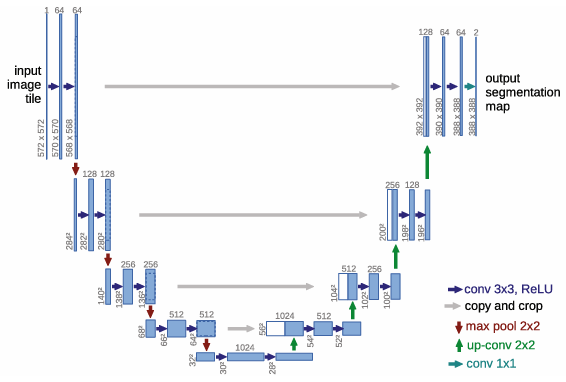
\includegraphics[width=0.75\linewidth]{../figures/UNet}
	\caption{U-Net architecture \cite{Ronneberger2015}.}
	\label{fig:UNet}
\end{figure}

The evaluation of all networks will be conducted using the Dice coefficient. The Dice coefficient is a commonly used metric for evaluating the similarity between two sets. In this context, it will be used for assessing the similarity between the segmentation mask generated by the segmentation network and the GT. The equation that describes the Dice coefficient can be seen in Equation \ref{eq:DiceCoefficient}, where $A$ is a set that represents the GT binary mask of one fluid and $B$ is another set that represents the predicted binary mask of the same fluid \cite{Shamir2019}. Considering $a_{i}$ and $b_{i}$ the binary pixels, the Dice coefficient can be rewritten as shown in Equation \ref{eq:DiceCoefficientPixels}. The network that performs the best will be selected to estimate the fluid volumes in the fluid volume estimation experiments.

\begin{equation}
	\text{Dice}(A, B) = \frac{2|A \cap B|}{|A| + |B|}
	\label{eq:DiceCoefficient}
\end{equation}

\begin{equation}
	\text{Dice}(A, B) = \frac{2\sum_{i} a_{i} b_{i}}{\sum_{i} a_{i} + \sum_{i} b_{i}}
	\label{eq:DiceCoefficientPixels}
\end{equation}

The loss function that regularized the training in the fluid segmentation experiments was the same as the one used in \textcite{Tennakoon2018}, whose segmentation model was previously implemented by the authors. This loss is described as seen in Equation \ref{eq:SegmentationLoss}, where $\lambda_{D}$ is the weight of the Dice component, $\mathcal{L}_{D}$, and $\lambda_{CE}$ is the weight of the cross-entropy component $\mathcal{L}_{CE}$, with both weights being 0.5.

\begin{equation}
	\mathcal{L} = \lambda_{D} \mathcal{L}_{D} + \lambda_{CE} \mathcal{L}_{CE}
	\label{eq:SegmentationLoss}
\end{equation}

The component $\mathcal{L_{D}}$ is the Dice loss of the foreground. This translates to how good the model is at detecting and segmenting the fluid present in the B-scans. For any image, where each pixel is associated with an index $j$, the loss can be described through Equation \ref{eq:SegmentationDice}, where $s_{j\overline{0}}$ is a binary variable that is 0 when the pixel $j$ belongs to the class 0 (background) and is 1 whenever the pixel $j$ belongs to any class that is not 0 (foreground). $p_{j\overline{0}}$ corresponds to the predicted probability of the pixel $j$ belonging to the foreground. The $\epsilon$ constant is a small value utilized to prevent division by zero.

\begin{equation}
	\mathcal{L}_{D} = 1 - \left( \frac{2 \sum_{j} s_{j\overline{0}} p_{j\overline{0}}}{\sum_{j} s_{j\overline{0}} + \sum_{j} p_{j\overline{0}} + \epsilon} \right)
	\label{eq:SegmentationDice}
\end{equation}

However, this loss component is not enough to correctly label the pixels in their respective classes and, for that reason, the cross-entropy component was used. Due to the large class imbalance in the images, with the background occupying the majority of them, the cross-entropy is balanced by taking into account the number of pixels belonging to each class. The cross-entropy is calculated for each pixel of index $j$ belonging to the image. Then, for each class, the cross-entropy of all pixels in the image is summed, before being divided by the number of pixels that belong to the class. The mean of the values obtained for each class result finally in $\mathcal{L}_{CE}$, as can be seen in Equation \ref{eq:SegmentationCE}.

\begin{equation}
	\mathcal{L}_{CE} = - \sum_{c \in C} \frac{1}{4}\left( \frac{1}{\sum_{j} s_{j,c}} \sum_{j} s_{j,c} \text{ln} p_{j,c} \right)
	\label{eq:SegmentationCE}
\end{equation}

\subsubsection{Experiment 1}
In the first experiment, the base U-Net model was trained to perform 2D multi-class segmentation of the retinal fluids in OCT volumes.
\par
This was the most extensive experiments, where many variables were tested. Different patch shapes, transformations, and hyperparameters were experimented, until the best training settings were determined. The best settings were then used in \ref{Experiment2} Experiment 2. All the experiments were done using the Adam optimizer \parencite{Kingma2017} with a learning rate of $2 \times 10^{-5}$.

\paragraph{Experiment 1.1}
The model was initially trained on patches of size 256 $\times$ 128 (H $\times$ W), following the same implementation as the one in \textcite{Tennakoon2018}. The extraction of patches aims at prioritizing the B-scan information relevant for the segmentation. To achieve this, the patches are not distributed uniformly. Instead, 10 patches are extracted from a random location inside the region of interest (ROI) of each image. The image's ROI is the part of the image where the entropy is above a determined threshold or where there retinal fluid is present. The patches are then augmented by a rotation between 0 and 10 degrees, and horizontal flipping. Of the patches with no fluid, 75\% of them were dropped. In Figure \ref{fig:FluidAndROI}, it is possible to see the overlaying of the fluid masks and the ROI, with a red bounding box signing a patch that would be used as input to train the U-Net.

\begin{figure}[!ht]
	\centering
	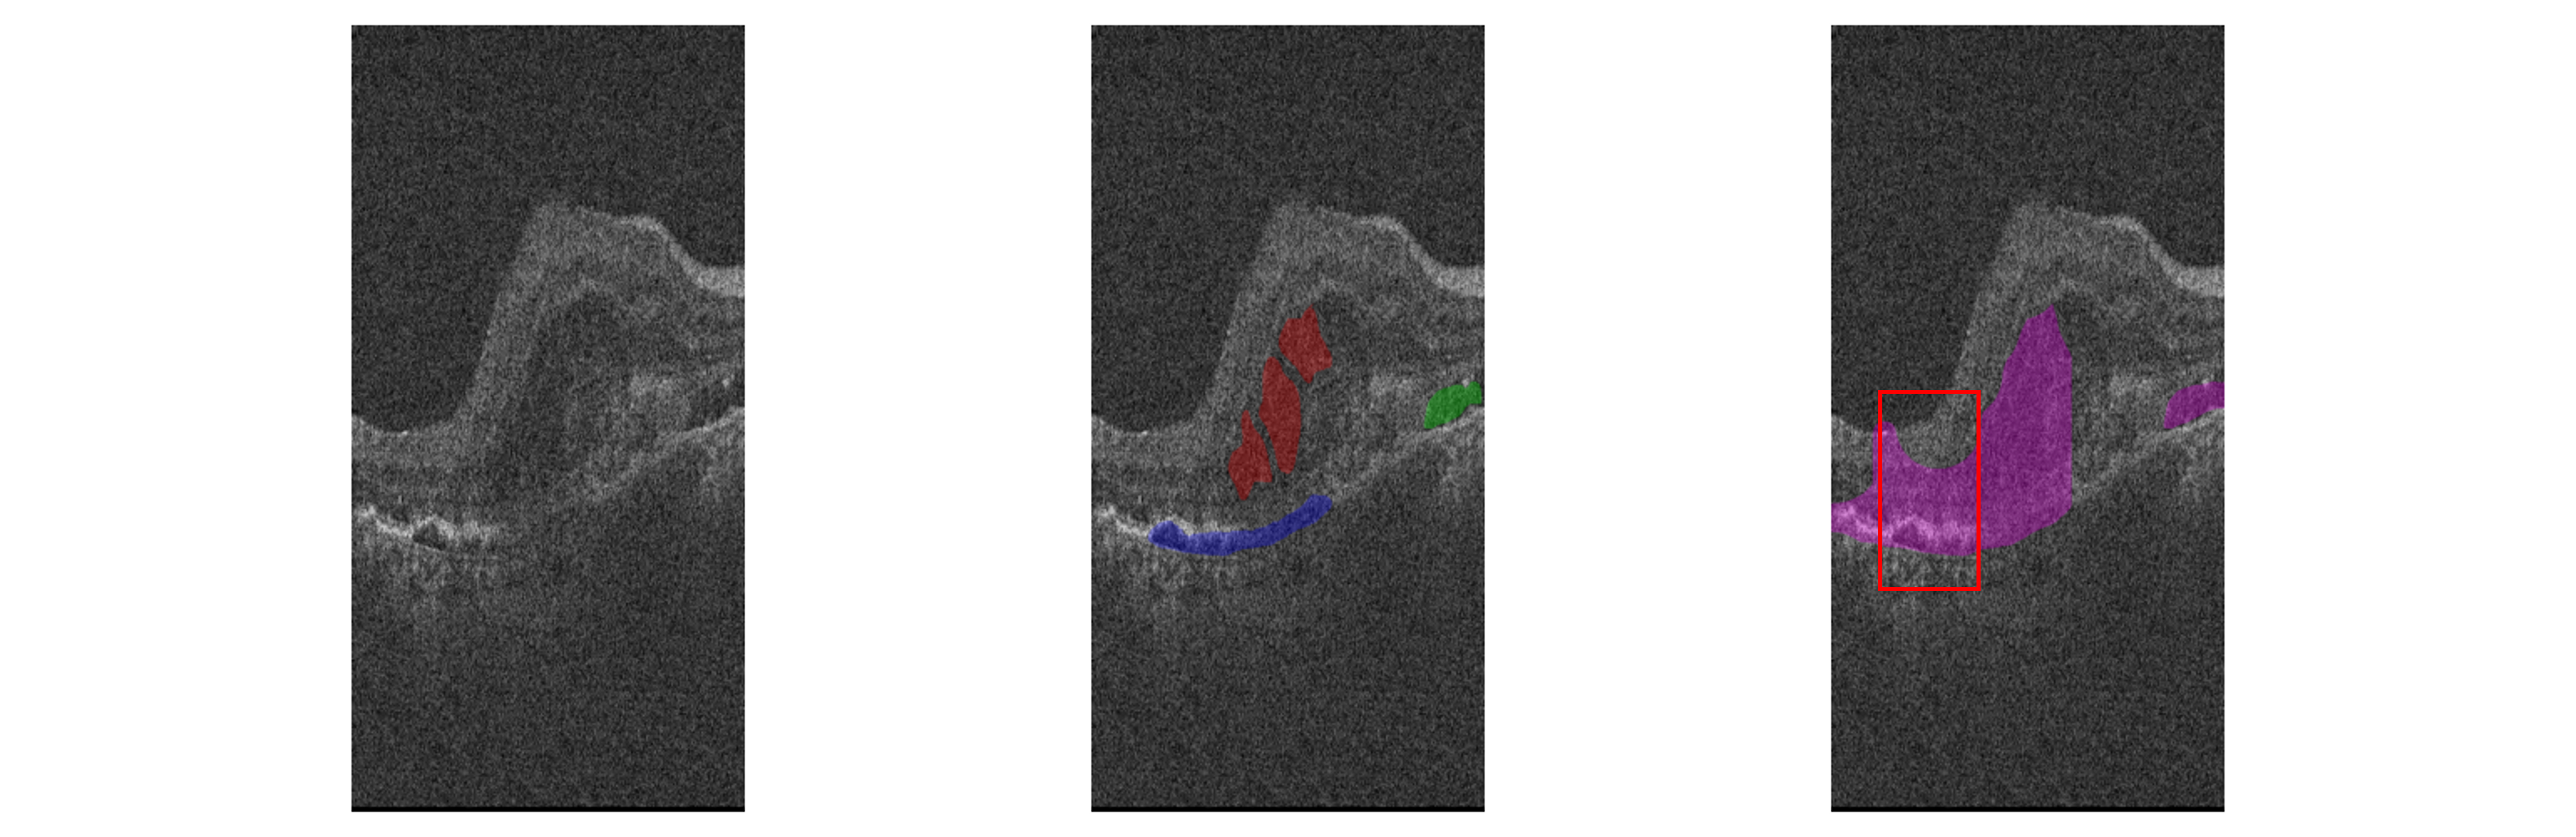
\includegraphics[width=1.0\linewidth]{../figures/FluidAndROI.png}
	\caption{Cirrus B-scan (left), fluid masks overlay (middle) with IRF in red, SRF in green, and PED in blue, and the ROI mask overlaid in purple (right).}
	\label{fig:FluidAndROI}
\end{figure}

\par
In the Experiment 1.1, two sets of four training runs were performed, using each fold as validation. In both sets, the conditions were exactly the same, except the input patches. This experiment aimed to understand the effect that the random patch extraction has on the model performances.

\paragraph{Experiment 1.2}
In Experiment 1.2, the patch shape was changed from 256 $\times$ 128 to 496 $\times$ 512. By using such shape, the model receives a larger context of the B-scan as input, allowing it to learn the anatomic references that characterize and limit the fluids.
\par
The patches used in this experiment were no longer randomly extracted from the ROI. Instead, the patches were extracted from top to bottom so that every section of the image would be present in at least one patch. In a Cirrus B-scan, with shape 1024 $\times$ 512, the first patch would correspond to section from $y=528$ to $y=1024$, while the second patch would be from $y=32$ to $y=528$. The last patch would then start on the bottom of the image, at $y=0$, to $y=496$. A representation of this process can be seen in Figure \ref{fig:BigPatchExtraction}. The patches are extracted from top to bottom so that the retina and the fluid would not be split in two patches, damaging the quality of the input data.

\begin{figure}[!ht]
	\centering
	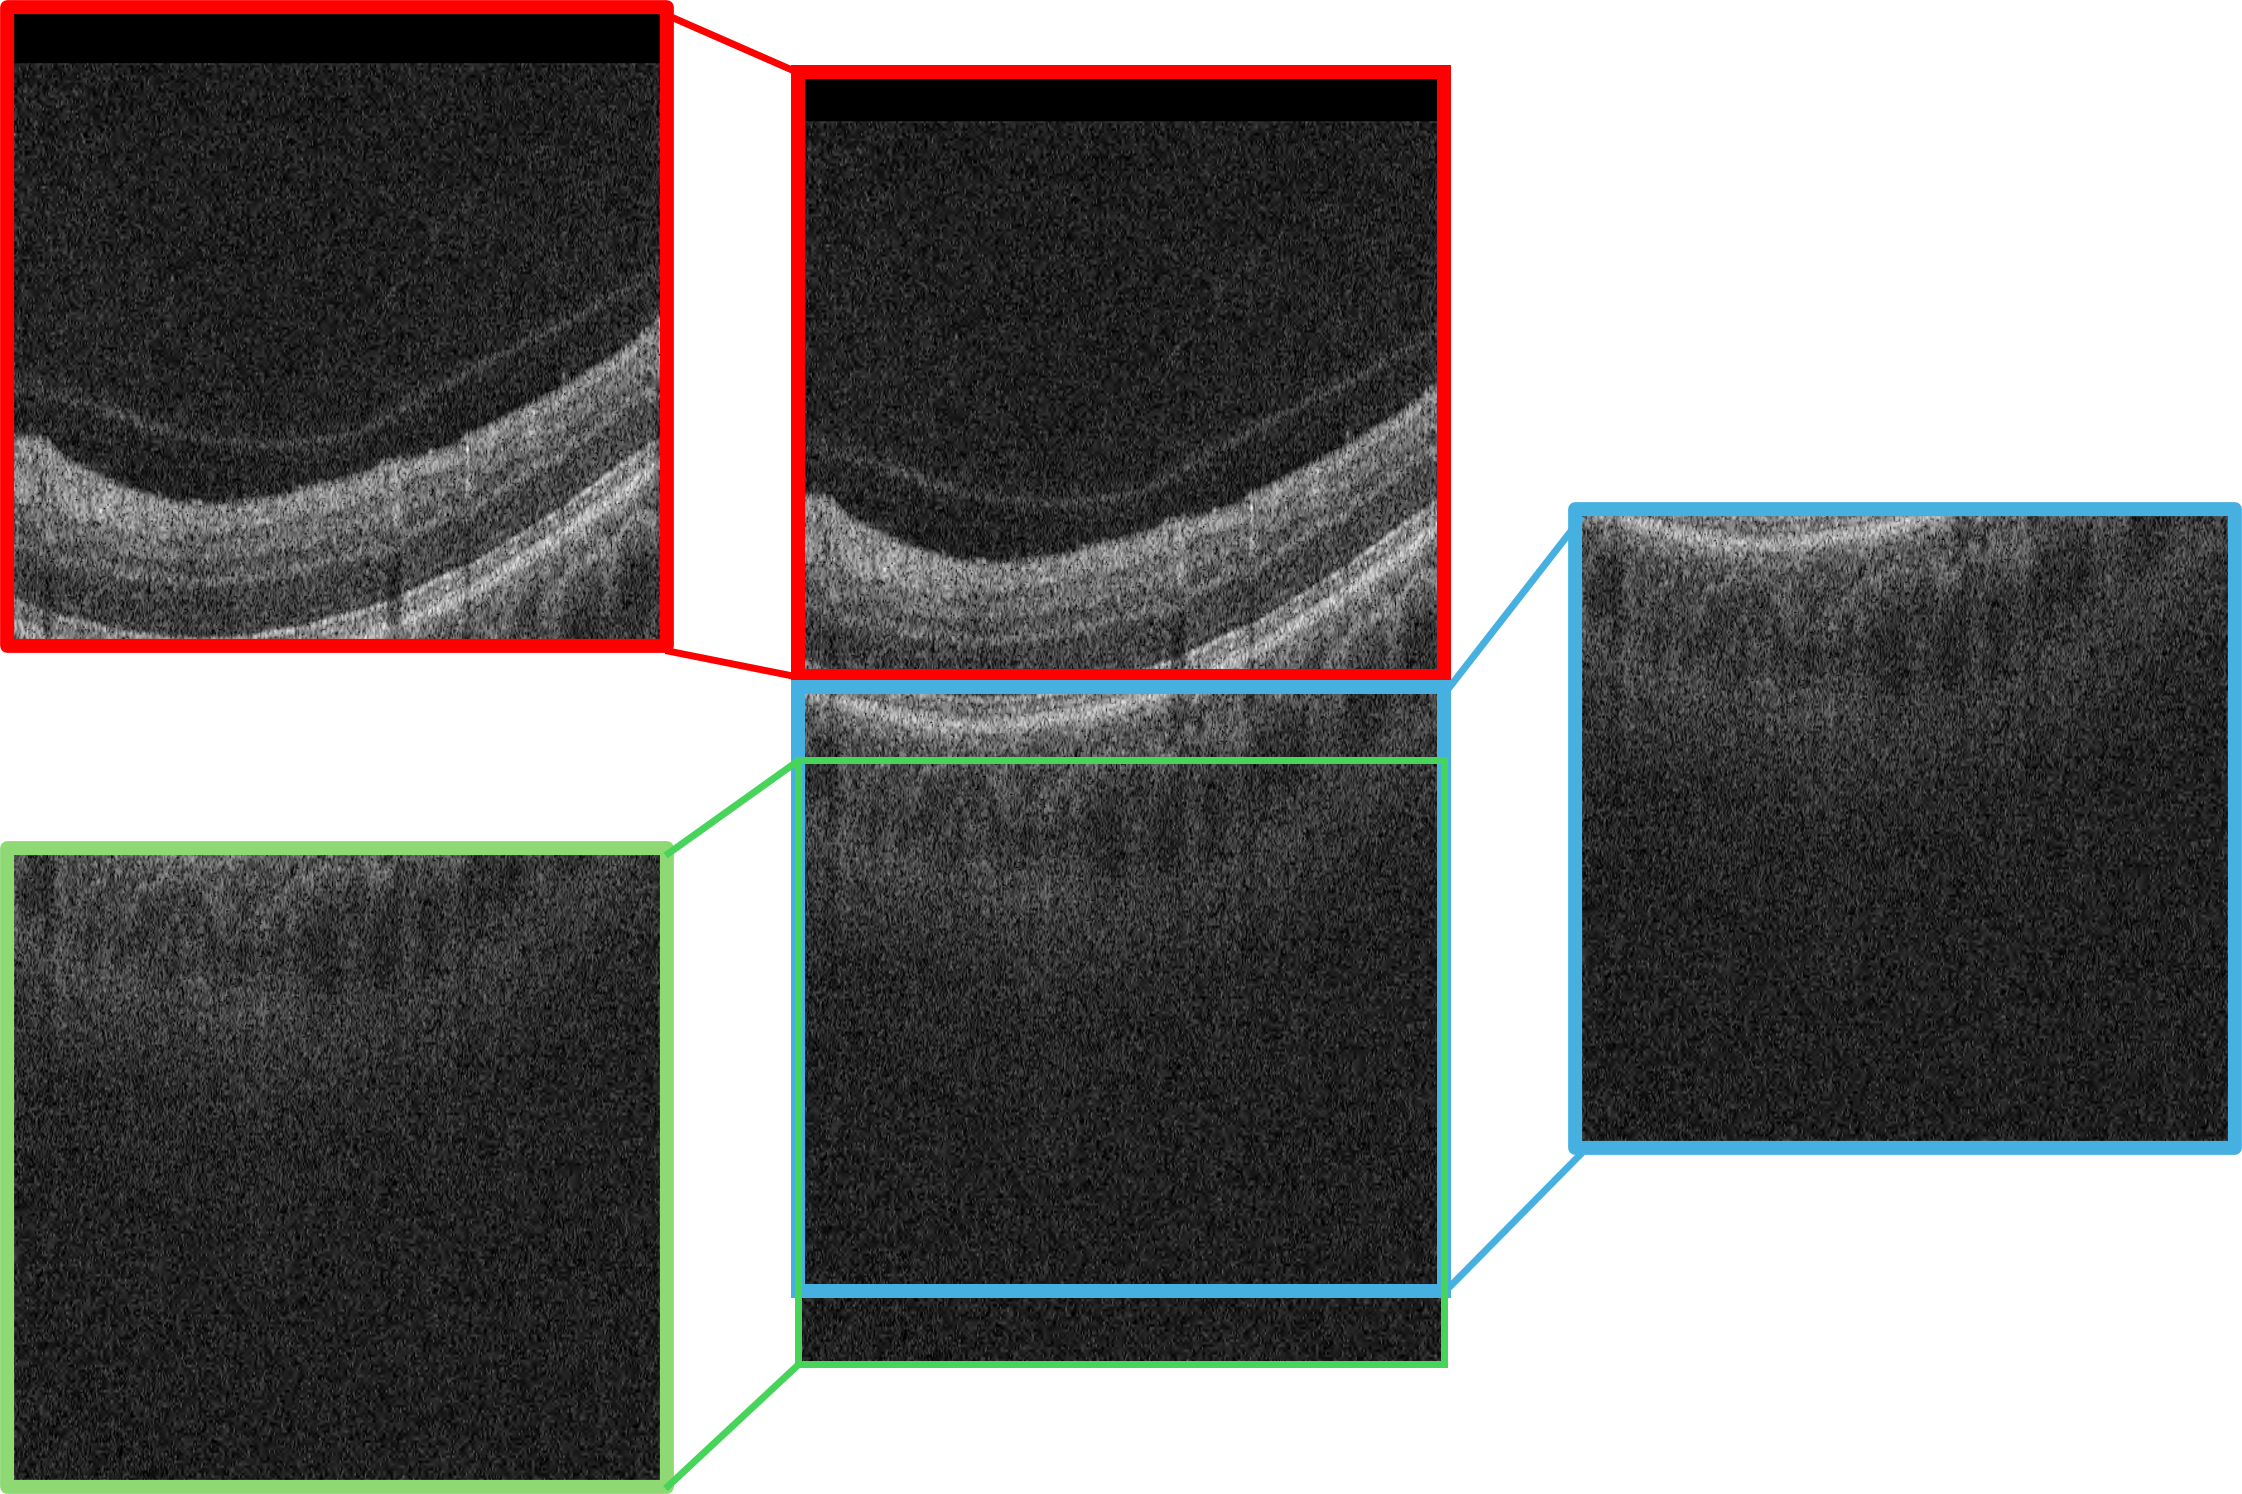
\includegraphics[width=0.5\linewidth]{../figures/BigPatchExtraction.png}
	\caption{Cirrus B-scan and its respective three patches of shape 496 $\times$ 512.}
	\label{fig:BigPatchExtraction}
\end{figure}

\subsubsection{Experiment 2}\label{Experiment2}
Similarly, in the second experiment, three U-Nets will be used for the segmentation task, one U-Net for each fluid type: one U-Net for the segmentation of IRF, one for SRF, and one for PED. This approach aligns with the methodology described in \textcite{Rahil2023, Padilla2022} and allows each network to specialize in the semantic segmentation of its fluid, improving the performance.

\subsubsection{Experiment 3}\label{Experiment3}
The subsequent experiment will be a repetition of the two previous experiments with an additional input. In papers such as \parencite{Tang2022, Lu2019, Rahil2023}, a relative distance map was used as an additional input channel to the network (see Figure \ref{fig:PreSegmentationAndFluidSegmentation}). This requires the initial delineation of the retina between the ILM and BM for which the retinal layer segmentation model developed by \textcite{Melo2023} will be utilized. Afterwards, the relative distance map will be extracted, considering only the mentioned layers, for each B-scan that compose the dataset. By providing information on the fluid location in the retina, this additional input significantly improved the performance of the segmentation models in \parencite{Tang2022, Lu2019, Rahil2023}.

\subsubsection{Experiment 4}\label{Experiment4}
The final experiment in the fluid segmentation task is inspired by the framework of \textcite{Tennakoon2018}. In this paper, 2.5D multi-class fluid segmentation is performed and patches of three consecutive slices are considered in the training phase. In order to keep the conditions equal across the experiments, the preprocessing and post-processing used in the original paper will not be performed. The network utilized in this framework, shown in Figure \ref{fig:TennakoonNetwork}, is similar to a U-Net, with the inclusion of batch normalization to improve training efficiency and dropout to prevent overfitting. With the inclusion of multiple slices in the input, it is expected an improvement on the segmentation.

\begin{figure}[!ht]
	\centering
	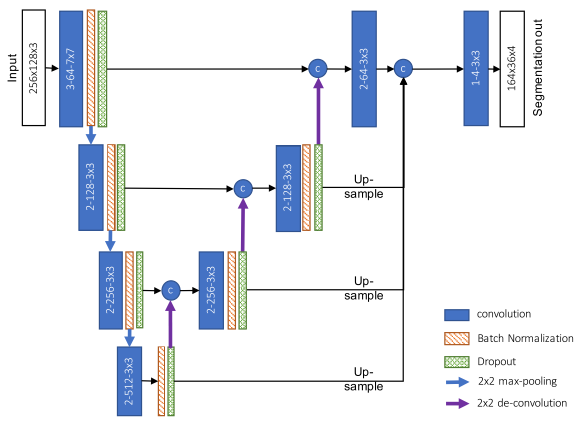
\includegraphics[width=0.7\linewidth]{../figures/TennakoonNetwork}
	\caption{The segmentation network in \cite{Tennakoon2018}.}
	\label{fig:TennakoonNetwork}
\end{figure}

\subsection{Intermediate Slice Synthesis}
The objective of the subsequent experiments is to improve the resolution between slices, thus approximating the fluid volume that will be estimated to the true value.
\par
The intermediate slices will be generated using the RETOUCH dataset. In this experiment, subvolumes that consist of overlapping triplets of consecutive slices, sampled with a step size of 1, will be used. The first and the last slice of these triplets will be used for the generation of the middle slice. Consequently, it is possible to evaluate the generated slice in comparison to the original one, as done in other examples of the literature. For each volume, the number of potential subsets is then determined to be $n-2$, where $n$ represents the number of slices within the same volume.
\par
As proposed in the fluid segmentation experiments, the split between the train, test, and validation sets will remain consistent. In the slice generation experiments, since the entire slice is necessary for generation and not just the fraction that contains fluid, the B-scans will not be patched.
\par
The generation of slices can be evaluated in specific metrics, as well as through qualitative assessment. To assess the efficacy of the generation model, the model utilized for fluid segmentation could be used for the estimation of the fluid's area in the generated image and to compare the resulting mask with the original image's mask. This comparison can be conducted using the Dice coefficient \parencite{Lopez2023} (see Equation \ref{eq:DiceCoefficientPixels}). However, this metric is insufficient for evaluating the generation performance, as it requires comparisons that encompass the entire slice and not just the fluid. Examples of such metrics include the mean absolute error (MAE) \parencite{Lopez2023, Wu2022, Zhang2022}, the peak signal-to-noise ratio (PSNR) \parencite{Xia2021, YChen2018, Sanchez2018, Fang2022, Nimitha2024, Kudo2019, You2020, Zhang2024, Zhang2022}, and the structural similarity index measure (SSIM) \parencite{YChen2018, Sanchez2018, Fang2022, Nimitha2024, Kudo2019, You2020, Zhang2024, Zhang2022}.

\paragraph{Experiment 5}
In the first experiment focused on intermediate slice synthesis, a GAN will be used. The underlying principle of a GAN, originally proposed by \textcite{Goodfellow2014}, is based on a competitive game between two networks. The generator network starts with the first and last slice of a subvolume, which is composed of three consecutive B-scans from an OCT scan, and aims to generate the intermediate slice. In contrast, the discriminator network is trained to distinguish between the generated and real slices. When the discriminator correctly labels generated slices as fake, the generator will be penalized, motivating it to fool the discriminator and consequently improving its generation, resulting in outputs more similar to the real inputs. However, the discriminator network loss also penalizes misclassifications, dependent on the probability of the prediction. As a result, as the generator improves, so does the discriminator \parencite{Goodfellow2020}. The overall framework for GANs is illustrated in Figure \ref{fig:GANFramework}.

\begin{figure}[!ht]
	\centering
	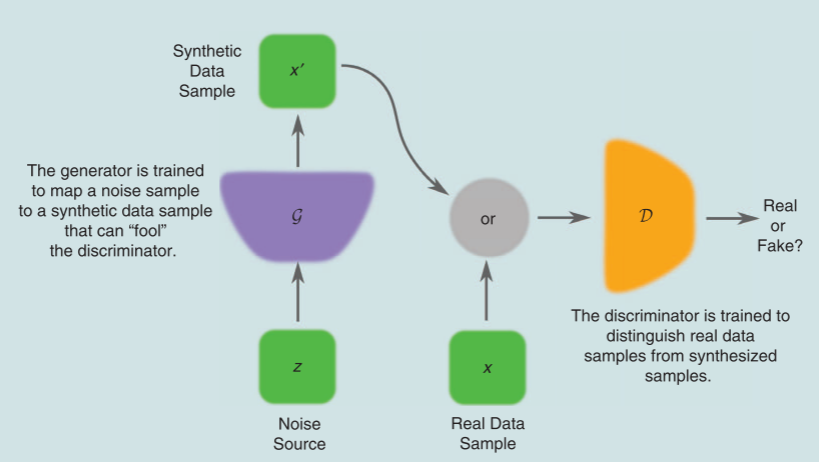
\includegraphics[width=0.7\linewidth]{../figures/GANFramework}
	\caption{Example of a GAN framework, where $\mathcal{D}$ is the discriminator and $\mathcal{G}$ is the generator \cite{Creswell2018}.}
	\label{fig:GANFramework}
\end{figure}

\paragraph{Experiment 6}
As in the previous experiment, the intermediate slice will be generated using the first and last slices of a subvolume that consists of three consecutive B-scans from an OCT scan. However, in this experiment, inspired by the work of \textcite{Nishimoto2024}, the intermediate slice will be generated using a U-Net. While the U-Net is more commonly applied in segmentation, as seen in the reviewed literature, \textcite{Nishimoto2024} apply it to generate the intermediate slices of a subvolume. The U-Net receives the edge slices as input and forces the output of the intermediate ones. In the paper \parencite{Nishimoto2024}, this was tested for three, four, and five slices. However, in this experiment it will be utilized to generate a single intermediate slice.

\subsection{Fluid Volume Estimation}
The estimation of fluid volume will be done once the optimal segmentation and intermediate slice generation models have been selected. Afterwards, the intermediate slice generation model will synthesize slices in the OCT volumes. The segmentation model will then be applied to both the unaltered volumes and the volumes with generated slices. 
\par
The area of each fluid in each OCT scan will be estimated considering the resolution of each OCT scan, which varies according to the device utilized to obtain the OCT volume. Afterwards, the area will be multiplied by the axial distance (half the axial distance to the previous slice plus half the axial distance to the following slice) to obtain the volume of fluid per slice. In the first and last slice of an OCT volume, the area will be multiplied by half of the axial distance (half the axial distance to the neighboring slice). The total volume of fluid in an OCT scan can be estimated by summing the fluid volumes of all individual B-scans. This allows the volume estimation of IRF, SRF, and PED, as well as the overall fluid volume in the OCT scan.

\paragraph{Experiment 7}
In this experiment, the fluid volumes will be calculated for the OCT scans without the generated slices. The best segmentation model will segment the fluid in three classes and the volume will be estimated for each class as described. The results from this experiment will allow the comparison with the values obtained in the following experiment, where slice generation will be used.

\paragraph{Experiment 8}
This experiment will consist of the fluid volume estimation in OCT scans with generated images. Similar to the previous experiment, the best segmentation model will predict the fluid masks and the fluid volume will be estimated. The values obtained will be compared with those calculated in the previous experiment. It is expected that the volumes will not vary more than one order of magnitude between experiments. In case a significant difference is observed, the generated images and their respective masks must be analyzed.